\documentclass[../../main/main.tex]{subfiles}
\graphicspath{{./figures/}}

\dominitoc
\faketableofcontents

% \renewcommand{\mtcSfont}{\small\bfseries}
% \renewcommand{\mtcSSfont}{\footnotesize}
\mtcsettitle{minitoc}{}
\mtcsetrules{*}{off}

\makeatletter
\renewcommand{\@chapapp}{Mécanique -- chapitre}
\renewcommand{\chaplett}{M}
\makeatother

% \toggletrue{student}
% \toggletrue{corrige}
% \renewcommand{\mycol}{black}
% \renewcommand{\mycol}{gray}

\hfuzz=5.002pt

\begin{document}
\setcounter{chapter}{1}

\settype{book}
\settype{prof}
\settype{stud}

\chapter{Dynamique du point en cartésiennes}

\vspace*{\fill}

\begin{tcn}(appl)<ctc>"somm"'t'{Sommaire}
	\let\item\olditem
	\vspace{-15pt}
	\minitoc
	\vspace{-25pt}
\end{tcn}

\begin{tcn}[sidebyside]
	(appl)<ctb>"how"'t'{Capacités exigibles}
	\begin{itemize}[label=\rcheck]
		\item Première loi de \textsc{Newton}~: décrire le mouvement relatif de
		      deux référentiels galiléens.
		\item Deuxième loi de \textsc{Newton}~: déterminer les équations du
		      mouvement d'un point matériel ou du centre de masse d'un système
		      fermé dans un référentiel galiléen.
		\item Troisième loi de \textsc{Newton}~: établir un bilan des forces sur
		      un système ou sur plusieurs systèmes en interaction et en rendre
		      compte sur un schéma.
		\item Exploiter la conservation de la masse pour un système fermé.
		\item Établir l'expression de la quantité de mouvement pour un système de
		      deux points sous la forme~: $\pf_{\Sc/\Rc}=m\vf_{\Gr/\Rc}$.
	\end{itemize}
	\tcblower
	\begin{itemize}[label=\rcheck]
		\item Force de gravitation. Modèle du champ de pesanteur uniforme au
		      voisinage de la surface d'une planète. Mouvement dans le champ de
		      pesanteur uniforme.
		\item Modèles d'une force de frottement fluide. Influence de la résistance
		      de l'air sur un mouvement de chute.
		\item Étudier le mouvement d'un système modélisé par un point matériel
		      dans un champ de pesanteur uniforme en l'absence de frottement.
		\item Exploiter, sans la résoudre analytiquement, une équation
		      différentielle~: analyse en ordres de grandeur, détermination de la
		      vitesse limite, utilisation des résultats obtenus par simulation
		      numérique. Écrire une équation adimensionnée.
	\end{itemize}
\end{tcn}

\vspace*{\fill}
\newpage
\vspace*{\fill}

%\vspace{-15pt}
\begin{tcn}[%
		sidebyside, fontupper=\small, fontlower=\small
	](appl)<ctb>"chek"'t'{L'essentiel}
	\tce{defi}
	% \tce{rapp}
	% \tce{loi}
	\tce{prop}
	\tce{demo}
	\tce{theo}
	\tce{prev}
	% \tce{coro}
	% \tce{inte}
	% \tce{impl}
	% \tce{tool}
	% \tce{nota}
	% \tce{appl}
	% \tce{rema}
	% \tce{exem}
	% \tce{ror}
	% \tce{impo}
	\tcblower
	% \tce{defi}
	\tce{rapp}
	% \tce{prop}
	% \tce{theo}
	\tce"Lois de \textsc{Newton}"{loi}
	% \tce{coro}
	% \tce{demo}
	% \tce{inte}
	% \tce{impl}
	% \tce{nota}
	\tce{appl}
	\tce{rema}
	\tce{exem}
	\tce{tool}
	\tce{ror}
	\tce{impo}
\end{tcn}

\vspace*{\fill}

\newpage

\section{Introduction}
% Dans ce chapitre nous nous intéressons à étudier les causes de la mise en
% mouvement d'un corps, représenté par un point matériel, et les mouvements qui en
% découlent.

\subsection{Inertie et quantité de mouvement}
Mettre en mouvement un corps revient à en \textbf{modifier la vitesse}. Il est
cependant plus facile de mettre en mouvement (ou arrêter le mouvement) certains
corps par rapport à d'autres. Ce phénomène s'appelle l'\textbf{inertie}, et est
proportionnel à la \textbf{masse d'un corps}.

\begin{tcb*}(defi){Inertie et quantité de mouvement}
	La résistance d'un corps matériel de masse $m$ à varier de vitesse est
	appelée \textbf{inertie}, quantifié par la \textbf{masse} et le
	\textbf{vecteur quantité de mouvement} du point matériel M du corps~:
	\psw{%
		\[
			\boxed{\pf\MRg(t) = m\vf\MRg(t)}
		\]
	}
	avec $\vf\MRg(t)$ le vecteur vitesse du point M dans le référentiel $\Rc$.
\end{tcb*}

Il est en effet plus difficile de déplacer une voiture à l'arrêt qu'un caddie à
l'arrêt, et inversement il est plus difficile d'arrêter une voiture qu'un
caddie. Dans l'analogie électromécanique, c'est l'inductance $L$ qui s'oppose à
la variation du courant quand $m$ s'oppose à la variation de la vitesse.

\subsection{Forces fondamentales}
Les causes du mouvement d'un corps sont appelées \textbf{forces}.
\begin{tcb}[sidebyside, righthand ratio=.3](defi){Forces}
	Les \textbf{forces} caractérisent les actions mécaniques sur un point matériel
	M. Ce sont des \textbf{vecteurs} et elles sont \textbf{indépendantes du
		référentiel}.
	\tcblower
	\tcbsubtitle{\fatbox{\textbf{Unité}}}
	\psw{%
		\[\boxed{\SI{1}{N} = \SI{1}{kg.m.s^{-2}}}\]
	}%
	\vspace{-15pt}
\end{tcb}
Il existe quatre de ces forces que l'on caractérise de «~fondamentales~», qui
permettent de classer les interactions physiques entre les systèmes~:

\begin{table}[htbp!]
	\centering
	\caption{Interactions fondamentales}
	\begin{tabularx}{\linewidth}{lYYYY}
		\toprule
		\diagbox[width=24.3mm,height=10mm]{\textbf{Caract.}}{\textbf{Type}} &
		\psw{\textbf{Faible}}                                               &
		\psw{\textbf{Forte}}                                                &
		\psw{\textbf{Électromag.}}                                          &
		\psw{\textbf{Grativationnelle}}
		\\
		\midrule
		Intensité                                                           &
		Faible                                                              &
		Très forte                                                          &
		Forte                                                               &
		Faible
		\\
		\addlinespace[0.5em]
		Portée                                                              &
		Extrême\mnt\ courte ($\approx \SI{e-18}{m}$)                        &
		Très courte ($\approx \SI{e-14}{m}$)                                &
		Longue                                                              &
		Très longue
		\\
		\addlinespace[0.5em]
		Agit sur                                                            &
		Fermions                                                            &
		Quarks et gluons                                                    &
		Particules chargées                                                 &
		Particules massives
		\\
		\addlinespace[0.5em]
		Conséquences                                                        &
		Désintégration radioactive, fusion nucléaire                        &
		Cohésion des nucléons                                               &
		Cohésion des matériaux, propriétés mécaniques                       &
		Poids, organisation cosmique
		\\
		\bottomrule
	\end{tabularx}
	\label{tab:int_fond}
\end{table}

\begin{tcb}(rapp){Interaction électrostatique}
	Avec l'interaction électrostatique, les particules de \textbf{même signe} se
	\textbf{repoussent}, tandis que celles de signes \textbf{opposées s'attirent}.
	Elle est responsable de la \textbf{cohésion des matériaux} et de leurs
	propriétés mécaniques (dureté, viscosité, propriétés chimiques…).
	\smallbreak
	La force d'interaction électrostatique causée par une particule de charge $q_A$
	sur une charge $q_B$ est~:
	\smallbreak
	\begin{isd}
		\psw{%
			\[
				\Ff_{e,\rm A\ra B} = \frac{1}{4\pi\ep_0} \frac{q_Aq_B}{\rm AB^2}\ur
				\qavec
				\ur = \frac{\vvr{AB}}{\rm AB}
			\]
		}%
		$\ur$ vecteur unitaire dirigé de A vers B.
		\tcblower
		\begin{center}
			\sswitch{
				\includegraphics[width=\linewidth]{fe_stud}
			}{
				\includegraphics[width=\linewidth]{fe_prof}
			}
			\vspace{-15pt}
			\captionof{figure}{Interaction électrostatique.}
		\end{center}
	\end{isd}
\end{tcb}

\begin{tcb}(rapp){Interaction gravitationnelle}
	Avec l'interaction gravitationnelle, la masse étant une grandeur positive,
	toutes les massives s'attirent entre elles. Elle prédomine à l'échelle
	astronomique.
	\smallbreak
	La force d'interaction gravitationnelle causée par une masse
	$m_A$ sur une masse $m_B$ est~:
	\smallbreak
	\begin{isd}
		\psw{%
			\[
				\Ff_{g,\rm A\ra B} = -\Gc \frac{m_Am_B}{\rm AB^2}\ur
				\qavec
				\ur = \frac{\vvr{AB}}{\rm AB}
			\]
		}%
		$\ur$ vecteur unitaire dirigé de A vers B.
		\tcblower
		\begin{center}
			\sswitch{
				\includegraphics[width=\linewidth]{fg_stud}
			}{
				\includegraphics[width=\linewidth]{fg_prof}
			}
			\vspace{-15pt}
			\captionof{figure}{Interaction gravitationnelle.}
		\end{center}
	\end{isd}
\end{tcb}

\section{Les trois lois de \textsc{Newton} (1687)}
\subsection{Principe d'inertie}

\begin{tcb*}(loi){Principe d'inertie}
	Il existe des référentiels appelés \textbf{référentiels galiléens} dans
	lesquels un point matériel M soumis à \textbf{aucune action mécanique} est
	\begin{itemize}
		\item \psw{soit \textbf{au repos}~;}
		\item \psw{soit en \textbf{translation rectiligne uniforme}.}
	\end{itemize}
	Ainsi, tout référentiel en translation rectiligne uniforme par rapport à un
	référentiel galiléen est galiléen.
\end{tcb*}

Il n'existe rigoureusement aucun référentiel galiléen, mais on peut en
considérer certains comme \textit{approximativement} galiléens lorsqu'on étudie
le problème sur \textbf{une durée assez courte} devant une durée typique du
système, afin que les effets de non-galiléeanité soient négligeables.

\begin{tcb*}[breakable](prop){Caractère galiléen des référentiels}
	Les référentiels fondamentaux sont \textit{supposés} galiléens si le mouvement
	est plus court que~:
	\begin{itemize}
		\item[b]{Référentiel héliocentrique}~:
		      un \textit{trajet significatif du Soleil dans la galaxie}, soit
		      \xul{\psw{\textbf{plusieurs millions d'années}}}~;
		\item[b]{Référentiel géocentrique}~:
		      un \textit{trajet significatif de la Terre autour du Soleil}, soit
		      \xul{\psw{\textbf{une année}}}~;
		\item[b]{Référentiels terrestres}~:
		      une \textit{rotation significative de la Terre}, soit
		      \xul{\psw{\textbf{une journée}}}.
	\end{itemize}
\end{tcb*}

\subsection{Principe fondamental de la dynamique}

C'est une des lois les plus importantes de la physique, permettant de
\textbf{relier le mouvement cinématique} (vitesse et associés) d'un corps en
\textbf{fonction de ses causes} (les forces extérieures).

\begin{tcb*}[list entry={\lte\theloi~:~Ppe. fondamental de la dynamique}]
	(loi){Principe fondamental de la dynamique}
	Dans un référentiel galiléen $\Rc$, l'évolution du vecteur
	\textbf{quantité de mouvement} $\pf\MRg(t)$ est reliée aux \textbf{forces
		extérieures} agissant sur le système~:
	\psw{%
		\[
			\boxed{\dv{\pf\MRg}{t} = \sum \Ff_{\ext\ra\Mr}}
		\]
	}
	Lorsque le \textbf{système est fermé} et donc la \textbf{masse est constante},
	on a $\forall t, m \dcancel{(t)} \Ra \pf\MRg(t) = m\vf\MRg(t)$, ainsi
	\psw{%
		\[
			\boxed{m\af\MRg(t) = \sum \Ff_{\ext\ra\Mr}}
		\]
	}
	avec $\af\MRg(t)$ le vecteur accélération du point M.
\end{tcb*}

\begin{tcb}(rema)<lftt>'l'{Mouvements de systèmes ouverts}
	Certains mouvements ne peuvent donc pas être traités avec cette dernière
	formulation s'ils s'accompagnent d'une variation de masse~:
	\begin{itemize}
		\item \psw{Le mouvement d'une fusée qui brûle son carburant puis abandonne
			      ses réservoirs~;}
		\item \psw{Le mouvement d'une goutte d'eau qui s'évapore lors de sa chute.}
	\end{itemize}
	Dans ces cas-là, on utilise la première formulation.
\end{tcb}

\subsection{Loi des actions réciproques}

\begin{tcb*}[sidebyside](loi){Loi des actions réciproques}
	Pour deux points M$_1$ et M$_2$ en interaction, la force exercée par le point
	1 sur le point 2 est égale à l'\textbf{opposé} de la force exercée par le
	point 2 sur le point 1~:
	\psw{%
		\[\boxed{\Ff_{1\ra2} = - \Ff_{2\ra1}}\]
	}%
	\vspace{-15pt}
	\tcblower
	\begin{center}
		\sswitch{
			\includegraphics[width=\linewidth]{loi3_stud}
		}{
			\includegraphics[width=\linewidth]{loi3_prof}
		}
		\vspace{-15pt}
		\captionof{figure}{Actions réciproques}
	\end{center}
\end{tcb*}

\section{Ensembles de points}
Aucun système n'est rigoureusement ponctuel, mais sous certaines conditions il
est possible d'étudier le mouvement d'un corps en tant que point matériel de
manière rigoureuse.

\subsection{Centre d'inertie}

\begin{tcb}(defi){Centre d'inertie}
	Le \textbf{centre d'inertie} ou \textbf{centre de gravité} G d'un ensemble
	de points matériels M$_i$ de masses $m_i$ est défini par~:
	\[
		\psw{%
			\boxed{\vvr{OG} = \sum_i \frac{m_i}{m_{\tot}} \vv{{\OMr}_i}}
		}
		\Lra
		\psw{%
			\boxed{\sum_i m_i \vvr{GM_i} = \of }
		}
		\qav
		\psw{%
			\text{O quelconque}
		}%
	\]
	Il s'agit du \textbf{barycentre} des points du système, \textbf{pondéré par
		leur masse}.
\end{tcb}

\begin{tcb}(exem)<lftt>{Centres de gravité}
	\begin{center}
		\sswitch{%
			\includegraphics[width=\linewidth]{cnt_grav_stud}
		}{%
			\includegraphics[width=\linewidth]{cnt_grav_prof}
		}%
		\vspace{-15pt}
		\captionof{figure}{Centres de gravités.}
	\end{center}
\end{tcb}

% Le centre d'inertie correspond au \textbf{centre d'équilibre gravitationnel}
% d'un ensemble de point. Ainsi, pour mettre une règle en équilibre
% horizontalement il faut la reposer en son milieu. Un marteau, en revanche, a son
% centre d'inertie bien plus proche de la masse que du milieu.

\begin{tcb}(demo){Centre d'inertie}
	\psw{%
		\begin{gather*}
			m_{\tot} = \sum_i m_i \Ra
			\sum_i m_i\vvr{OG} = \sum_i m_i\vv{\OMr_i}
			\Lra
			\of                   = \sum_i m_i \left( \vv{\OMr_i} - \vvr{OG} \right)
		\end{gather*}
		Or, comme $\vv{\OMr_i} - \vvr{OG} = \vvr{GO} + \vv{\OMr_i} = \vv{\rm
				GM_i}$, on aura bien~:
		\[
			\boxed{\sum_i m_i\vv{{\rm GM}_i} = \of}
		\]
	}
\end{tcb}

\begin{tcb}[breakable](appl)<lftt>'l'{Centres d'inertie}
	Soient 2 masses placées en A et en B. Déterminer la position de G en
	calculant $\vvr{AG}$ dans les deux cas suivants~:
	\begin{tasks}(2)
		\task[\fbox{1}]
		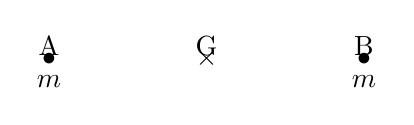
\begin{tikzpicture}[anchor=base, baseline]
			\coordinate (A) at (-2,0);
			\coordinate (B) at (2,0);
			\coordinate (G) at (0,0);
			\node[] at (A) {$\bullet$};
			\node[below] at (A) {$m$};
			\node[above=.1] at (A) {A};
			\node[] at (B) {$\bullet$};
			\node[below] at (B) {$m$};
			\node[above=.1] at (B) {B};
			\node[] at (G) {$\times$};
			\node[above=.1] at (G) {G};
		\end{tikzpicture}
		\task[\fbox{2}]
		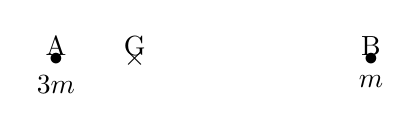
\begin{tikzpicture}[anchor=base, baseline]
			\coordinate (A) at (-2,0);
			\coordinate (B) at (2,0);
			\coordinate (G) at (-1,0);
			\node[] at (A) {$\bullet$};
			\node[below] at (A) {$3m$};
			\node[above=.1] at (A) {A};
			\node[] at (B) {$\bullet$};
			\node[below] at (B) {$m$};
			\node[above=.1] at (B) {B};
			\node[] at (G) {$\times$};
			\node[above=.1] at (G) {G};
		\end{tikzpicture}
	\end{tasks}
	\tcblower
	\begin{enumerate}[label=\sqenumi]
		\item[m] \psw{%
			      \begin{gather*}
				      \beforetext{O = A $\Ra$}
				      \vvr{AG} = \frac{m}{2m} \vvr{AB} + \of
				      \Lra
				      \boxed{\vvr{AG} = \frac{1}{2}\vvr{AB}}
			      \end{gather*}
		      }%
		      \vspace{-15pt}
		\item[m] \psw{%
			      \begin{gather*}
				      \beforetext{De même,}
				      \vvr{AG} = \frac{3m}{4m}\vvr{AB} + \of
				      \Lra
				      \boxed{\vvr{AG} = \frac{1}{4}\vvr{AB}}
			      \end{gather*}
		      }%
		      \vspace{-15pt}
	\end{enumerate}
\end{tcb}

\begin{tcb}(rema)<lftt>{Solides continus}
	Cette définition peut être étendue aux solides qui peuvent être vus comme un
	ensemble infini de points infiniment proches. Dans ce cas, la somme discrète
	devient une intégrale.
\end{tcb}

\subsection{Quantité de mouvement d'un ensemble de points}

% On souhaiterait pouvoir étudier un ensemble de points comme le mouvement d'un
% point unique, comme le centre d'inertie. Pour cela, il faut étudier la quantité
% de mouvement d'un ensemble de points.

\begin{tcb*}(defi){$\protect\pf$ d'un ensemble de points}
	Le vecteur quantité de mouvement d'un ensemble $\Sc$ de points matériels
	M$_i$ de masses $m_i$ est la somme des quantités de mouvement de chacun des
	points~:
	\psw{%
		\[
			\boxed{\pf_{\Sc/\Rc}(t) = \sum_i m_i \vf_{\Mr_i/\Rc}(t)}
		\]
	}%
	\vspace{-15pt}
\end{tcb*}

\begin{tcb*}(prop){$\protect\pf_{\Sc}$ et centre d'inertie}
	La quantité de mouvement d'un ensemble de points est la quantité de
	mouvement d'un point matériel placé en $G$ et de masse $m_{\tot}$~:
	\psw{%
		\[
			\boxed{\pf_{\Sc/\Rc}(t) = m_{\tot}\vf_{\Gr/\Rc}(t)}
		\]
	}%
	\vspace{-25pt}
	\begin{center}
		\textbf{Tout se passe comme si la masse était concentrée en G.}
	\end{center}
\end{tcb*}

\begin{tcb*}(demo){$\protect\pf_{\Sc}$ et centre d'inertie}
	Pour que les choses soient simples, il faudrait donc que $\pf_{\Sc/\Rc}(t)$
	soit relié au centre d'inertie. Or,
	\psw{%
		\[
			\vf_{\Gr/\Rc}(t) = \dv{\vvr{OG}}{t} = \frac{1}{m_{\tot}}
			\underbracket[1pt]{\sum_i m_i \dv{{\OM}_i}{t}}_{\pf_{\Sc/\Rc}(t)}
			\Lra
			\boxed{\pf_{\Sc/\Rc}(t) = m_{\tot}\vf_{\Gr/\Rc}(t)}
		\]
	}%
	\vspace{-15pt}
\end{tcb*}

\subsection{Théorème de la résultante cinétique}
Si on peut étudier la cinématique d'un corps par l'étude de son centre de
gravité, comment les forces interviennent-elles sur cet ensemble de points~?

\begin{tcb*}(prev){Résultante cinétique}
	Considérons pour simplifier un système de deux points M$_1$ et M$_2$ de masses
	$m_1$ et $m_2$ en mouvement dans un référentiel galiléen. On peut appliquer le
	principe fondamental de la dynamique à chacun d'entre eux~:
	\[
		\psw{%
			\dv{\pf_{\Mr_1/\Rc}}{t} = \Ff_{\Mr_2\ra\Mr_1} + \Ff_{\ext\ra\Mr_1}
		}%
		\qet
		\psw{%
			\dv{\pf_{\Mr_2/\Rc}}{t} = \Ff_{\Mr_1\ra\Mr_2} + \Ff_{\ext\ra\Mr_2}
		}%
	\]
	avec deux types de forces~: les \textbf{forces intérieures} du système, ici
	celles exercées par M$_2$ sur M$_1$, et les \textbf{forces extérieures},
	c'est-à-dire toutes les autres. Ainsi, avec la définition de la quantité de
	mouvement d'un ensemble de points,
	\psw{%
		\[
			\dv{\pf_{\Sc/\Rc}}{t} =
			\dv{\pf_{\Mr_1/\Rc}}{t} + \dv{\pf_{\Mr_2/\Rc}}{t} =
			\underbracket[1pt]{\Ff_{\Mr_1\ra\Mr_2}+\Ff_{\Mr_2\ra\Mr_1}}_{= \of
				\text{ d'après la 3ème loi}} + \Ff_{\ext\ra\Mr_1} + \Ff_{\ext\ra\Mr_2}
			\qed
		\]
	}%
\end{tcb*}

\begin{tcb*}(theo){Résultante cinétique}
	Le \textbf{PFD pour un point} se transpose à un \textit{ensemble de points} en
	prenant pour \textbf{point matériel} le \textbf{centre d'inertie G} affecté de
	la masse totale $m_{\tot}$ du système, en ne considérant que les
	\textbf{forces extérieures} s'appliquant à l'ensemble~:
	\begin{gather*}
		\beforetext{TRC~:}
		\psw{%
			\boxed{m_{\tot}\dv{\vf_{\Gr/\Rc}}{t} = \sum \Ff_{\ext\to\Sc}}
		}%
	\end{gather*}
\end{tcb*}

\begin{tcb*}(ror){Conclusion ensemble de points}
	Le mouvement du centre de gravité n'est affecté que par les forces extérieures
	au système. Ainsi, dans la suite, on étudiera le \textbf{mouvement du centre
		de gravité}, de masse $m_{\tot}$, soumis aux \textbf{forces extérieures} au
	système.
\end{tcb*}

\subsection{Méthode générale de résolution en mécanique}
\begin{tcb*}(tool){Étapes de résolution}
	\begin{enumerate}[label=\sqenumi]
		\item[b]{Système}~: quel est l'objet en mouvement, dans quel
		      référentiel étudie-t-on le mouvement~?

		\item[b]{Schéma}~: faire un schéma du problème dans une \textbf{situation
			      quelconque}\ftn{On ne fait \textbf{jamais} de schéma à l'équilibre
			      ou à des angles particuliers ($\ang{45;;}$ par exemple)}.

		\item[b]{Modélisation}~: donner le repère, détailler le repérage, les
		      conditions initiales, les représenter sur le schéma et \textit{définir
			      les notations} nécessaires.

		\item[b]{Bilan des forces}~: faire le bilan \textbf{dans le repère} choisi,
		      \textbf{les représenter} sur le schéma.

		\item[b]{Deuxième loi de \textsc{Newton}}~: appliquer le PFD/TRC au système.

		\item[b]{Équations scalaires}~: donner les trois équations $\ddot{x}(t)$,
		      $\ddot{y}(t)$ et $\ddot{z}(t)$.

		\item[b]{Répondre aux questions}~: le plus souvent, obtenir les équations
		      horaires $x(t)$, $y(t)$ et $z(t)$.
	\end{enumerate}
\end{tcb*}

% \begin{tcb}*(expe)<itc>"trans"{Transition}
% 	Avec ces outils, voyons maintenant quelques forces et situations usuelles
% 	que l'on rencontrera en dynamique.
% \end{tcb}

\section{Forces usuelles}
\subsection{Le poids}
% \subsubsection{Définition}

\begin{tcb*}[sidebyside](defi){Poids et pesanteur}
	Dû à l'attraction gravitationnelle de la Terre, un corps de masse $m$ à sa
	surface subit une force que l'on appelle le \textbf{poids}, telle que~:
	\psw{%
		\[\boxed{\Pf = m\gf = -mg\uz}\]
	}%
	avec $\gf$ le vecteur \textbf{accélération de la pesanteur}, de norme $g =
		\norm{\gf} = \SI{9.81}{m.s^{-2}}$ et dirigé \textbf{verticalement vers le
		sol}.
	\tcblower
	Par définition de l'interaction gravitationnelle, on a
	\psw{%
	\[\boxed{\gf = -\Gc \frac{m_T}{R_T{}^2}\uz}\]
	}%
	avec $m_T$ et $R_T$ la masse et le rayon de la Terre, $\Gc$ la constante
	gravitationnelle, et $\uz$ vertical ascendant.
\end{tcb*}

% \subsubsection{La chute libre}
\begin{tcb*}(defi)<lftt>'l'{Chute libre, flèche et portée}
	Un système en \textbf{chute libre} pure ne subit \textbf{que son poids}. On
	appelle \textbf{portée} d'un tir la \textbf{distance horizontale} entre
	l'origine et le point d'impact, et \textbf{flèche} la \textbf{hauteur
		maximale} atteinte par le projectile.
\end{tcb*}

\begin{tcb*}(prop){Tir en chute libre}
	Soit un corps tiré à la surface de la Terre à altitude nulle, soumis
	uniquement à son poids, lancé à la vitesse $\vfo$ faisant un angle $\alpha$
	avec le sol. Alors~:
	\begin{enumerate}
		\item La masse du corps n'intervient pas dans l'expression de son
		      accélération~;
		\item La trajectoire qu'il forme est une parabole~;
		\item La portée maximale est atteinte pour $\alpha = \xul{\psw{\pi/4}}$~;
		\item La flèche maximale est atteinte pour $\alpha = \xul{\psw{\pi/2}}$~;
		\item Le temps de vol est maximal pour $\alpha = \xul{\psw{\pi/2}}$.
	\end{enumerate}
\end{tcb*}

\begin{tcb*}[breakable](demo){Tir en chute libre}
	\begin{enumerate}
		\item On établit le système pour relier l'accélération aux causes
		      extérieures~:
		      \smallbreak
		      \begin{minipage}[t]{0.50\linewidth}
			      \begin{enumerate}[label=\sqenumi]
				      \item[b]{Système}~: \psw{\{balle\}}%
				      \item[b]{Schéma}.
				      \item[b]{Modélisation}.
				            \begin{itemize}
					            \item[b]{Référentiel}~: \psw{$\Rc\ind{labo}$ supposé
						                  galiléen}
					            \item[b]{Repère}~: \psw{$(\Or, \ux, \uy, \uz)$ (voir
						                  schéma)}
					            \item[b]{Repérage}~:
				            \end{itemize}
			      \end{enumerate}
		      \end{minipage}
		      \hfill
		      \begin{minipage}[t]{0.45\linewidth}
			      \begin{center}
				      \vspace{-12pt}
				      \sswitch{%
					      \includegraphics[width=\linewidth]{cl_ssf_stud}
				      }{%
					      \includegraphics[width=\linewidth]{cl_ssf_prof}
				      }%
				      \vspace{-15pt}
				      \captionof{figure}{Chute libre.}
			      \end{center}
		      \end{minipage}
		      \begin{enumerate}[label=\sqenumi, start=4]
			      \item{}[]
			            \begin{itemize}
				            \item{}[]
				                  \vspace{-20pt}
				                  \psw{%
					                  \begin{align*}
						                  \OM(t) & = x(t)\ux + y(t)\uy + z(t)\uz
						                  \\
						                  % \quad ; \quad
						                  \vf(t) & = \xp(t)\ux + \yp(t)\uy + \zp(t)\uz
						                  \\
						                  % \quad ; \quad
						                  \af(t) & = \xpp(t)\ux + \ypp(t)\uy + \zpp(t)\uz
					                  \end{align*}
				                  }%
				                  \vspace{-25pt}
				            \item[b]{Conditions initales}~:
				                  \[
					                  \psw{%
						                  \OM(0) = \of
					                  }
					                  \qet
					                  \psw{%
						                  \vf(0) = v_0\cos (\alpha)\ux + v_0\sin (\alpha)\uy
					                  }%
				                  \]
			            \end{itemize}
			      \item[b]{Bilan des forces}~:
			            \psw{%
				            Ici, seul le poids s'applique~:
				            \[
					            \begin{array}{ll}
						            \textbf{Poids} & \Pf = m\gf = -mg\uy
					            \end{array}
				            \]
			            }%
			            \vspace{-25pt}
			      \item \leftcenters{\textbf{PFD.}}{\psw{$m\af(t) = \Pf$}}
			      \item[b]{Équations scalaires}~: on projette sur les axes~:
			            \psw{%
				            \[
					            \left\{
					            \begin{array}{l}
						            m\ddot{x}(t) = 0   \\
						            m\ddot{y}(t) = -mg \\
						            m\ddot{z}(t) = 0
						            \quad \text{ignoré dans la suite}
					            \end{array}
					            \right.
					            \quad \Lra \quad
					            \left\{
					            \begin{array}{l}
						            \ddot{x}(t) = 0 \\
						            \ddot{y}(t) = -g
					            \end{array}
					            \right.
				            \]
			            }%
			            On remarque donc bien que l'accélération ne dépend pas de la
			            masse~; ainsi, \textit{sans frottements}, \textbf{tous les
				            corps chutent à la même
				            vitesse}\ftn{\url{https://www.youtube.com/watch?v=E43-CfukEgs}}.
		      \end{enumerate}
		\item On commence par trouver les équations horaires. Pour cela, on
		      intègre l'accélération pour obtenir la vitesse~:
		      \[
			      \psw{%
				      \left\{
				      \begin{array}{l}
					      \dot{x}(t) = K_1 \\
					      \dot{y}(t) = -gt + K_2
				      \end{array}
				      \right.
			      }
			      \qor
			      \psw{%
				      \left\{
				      \begin{array}{l}
					      \dot{x}(0) = v_0\cos\alpha = K_1 \\
					      \dot{y}(0) = v_0\sin\alpha = K_2
				      \end{array}
				      \right.
			      }
			      \Ra
			      \psw{%
				      \boxed{
					      \left\{
					      \begin{array}{l}
						      \dot{x}(t) = v_0\cos\alpha \\
						      \dot{y}(t) = -gt + v_0\sin\alpha
					      \end{array}
					      \right.
				      }
			      }
		      \]
		      De même pour les équations horaires du mouvement~:
		      \[
			      \psw{%
				      \left\{
				      \begin{array}{l}
					      x(t) = v_0t\cos\alpha + C_1 \\
					      y(t) = \DS -\frac{1}{2}gt^2 + v_0t\sin\alpha + C_2
				      \end{array}
				      \right.
			      }
			      \qor
			      \psw{%
				      \left\{
				      \begin{array}{l}
					      x(0) = 0 = C_1 \\
					      y(0) = 0 = C_2
				      \end{array}
				      \right.
			      }
			      \Ra
			      \psw{%
				      \boxed{
					      \left\{
					      \begin{array}{l}
						      x(t) = v_0t\cos\alpha \\
						      y(t) = \DS -\frac{1}{2}gt^2 + v_0t\sin\alpha
					      \end{array}
					      \right.
				      }
			      }
		      \]
		      \begin{isd}
			      Si on cherche la trajectoire, il s'agit alors d'obtenir la courbe
			      $y(x)$ décrite dans le plan $xy$, c'est-à-dire éliminer le temps $t$.
			      À partir de l'équation horaire sur $\ux$, on a
			      \psw{%
				      \begin{align*}
					      t    & =
					      \frac{x}{v_0\cos\alpha}
					      \\\Lra
					      y(x) & =
					      - \frac{1}{2}g \frac{x^2}{v_0{}^2\cos^2\alpha} + v_0\sin\alpha
					      \frac{x}{v_0\cos\alpha}
					      \\\Lra
					      \Aboxed{%
					      y(x) & =
					      - \frac{g}{2v_0{}^2\cos^2\alpha}x^2 + x\tan\alpha
					      }%
					      \qed
				      \end{align*}
			      }%
			      \vspace{-15pt}
			      \tcblower
			      \begin{center}
				      \sswitch{%
					      \includegraphics[width=\linewidth]{cl_ssf-traj_stud}
				      }{%
					      \includegraphics[width=\linewidth]{cl_ssf-traj_prof}
				      }%
				      \captionof{figure}{Tir en chute libre.}
				      \label{fig:cl_ssf-traj}
			      \end{center}
		      \end{isd}
		\item On trouve $x_P$ tel que~:
		      \psw{%
			      \begin{gather*}
				      y(x_P) = 0
				      \Lra
				      \underbracket[1pt]{x_P}_{\neq 0}
				      \left(- \frac{g}{2v_0{}^2\cos^2\alpha}x_P + \tan\alpha\right) = 0
				      \Lra
				      - \frac{g}{2v_0{}^2\cos^2\alpha}x_P + \tan\alpha = 0
				      \\
				      \Lra
				      x_P = \frac{2v_0{}^2\cos^2\alpha}{g}\tan\alpha =
				      \frac{2v_0{}^2\cos^{\cancel{2}}\alpha}{g}
				      \frac{\sin\alpha}{\cancel{\cos\alpha}} =
				      \frac{v_0{}^2}{g}\times 2\sin\alpha\cos\a
				      \\
				      \Lra
				      \boxed{x_P = \frac{v_0{}^2}{g}\sin(2\a)}
				      \qet
				      x_{P,\rm max} \qMath{pour} \sin(2\a) = 1 \Lra
				      \boxed{\alpha\ind{max} = \frac{\pi}{4}}
			      \end{gather*}
		      }%
		\item On trouve $y_F$ quand la vitesse \textbf{verticale} s'annule,
		      $\dot{y}(t_F) = 0$~:
		      \psw{%
			      \begin{gather*}
				      \yp(t_F) = -gt_F + v_0\sin\alpha = 0
				      \Lra
				      t_F = \frac{v_0\sin\a}{g}
				      \\\Ra
				      y(t_F) = -\frac{1}{2}g \left( \frac{v_0\sin\a}{g} \right)^2 +
				      v_0\sin\a\times \frac{v_0\sin\a}{g}
				      \\\Lra
				      \boxed{y_F = \frac{v_0{}^2}{2g}\sin^2\alpha}
				      \qet
				      y_{F,\rm max} \qMath{pour} \sin^2(\a) = 1 \Lra
				      \boxed{\alpha\ind{max} = \frac{\pi}{2}}
			      \end{gather*}
		      }%
		      \vspace{-15pt}
		\item Le temps de vol est le temps pour lequel le projectile retombe au
		      sol, c'est-à-dire $t(x_P)$~:
		      \psw{%
			      \begin{gather*}
				      \Lra
				      t(x_P) = \frac{\frac{v_0{}^{\cancel{2}}}{g}\times
				      2\sin\a\bcancel{\cos\a}}{\cancel{v_0}\bcancel{\cos\a}}
				      \\\Lra
				      \boxed{t(x_P) = 2 \frac{v_0}{g}\sin\a}
				      \qet
				      t_{x_P,\rm max} \qMath{pour} \sin(\a) = 1 \Lra
				      \boxed{\alpha\ind{max} = \frac{\pi}{2}}
				      \qed
			      \end{gather*}
		      }%
	\end{enumerate}
\end{tcb*}

\subsection{Poussée d'\textsc{Archimède}}
\begin{tcb*}(defi){Poussée d'\textsc{Archimède}}
	Lorsqu'un objet est dans un fluide, il subit une force nommée
	\textbf{poussée d'\textsc{Archimède}} et égale à l'opposé du poids du fluide
	déplacé. Elle est parfois notée $\Pif$ ou $\Ff_A$, et on a~:
	\psw{%
		\[\boxed{\Ff_A = -\rho\ind{fluide}V\ind{immergé}\gf}\]
	}%
	avec $\rho\ind{fluide}$ la masse volumique du fluide et $V\ind{immergé}$ le
	volume de l'objet qui est dans le fluide.
\end{tcb*}

\begin{tcb}[breakable](appl)<lftt>'l'{Glaçon immergé}
	Quelle est la proportion immergée d'un glaçon~?
	\smallbreak
	On donne $\rho\ind{eau} = \SI{1.00e3}{kg.m^{-3}}$ et $\rho\ind{glace} =
		\SI{9.17e2}{kg.m^{-3}}$.
	\tcblower
	\begin{isd}[righthand ratio=.22]
		\psw}
			\end{gather*}
		}%
		\vspace{-15pt}
		\tcblower
		\begin{center}
			\sswitch{
				\includegraphics[width=\linewidth, draft=true]{glacon}
			}{
				\includegraphics[width=\linewidth]{glacon}
			}
			\vspace{-15pt}
			\captionof{figure}{}
		\end{center}
	\end{isd}
	\vspace{-15pt}
	% \psw{%
	% 	On observe également qu'un objet \textbf{plus dense} que le fluide aura
	% 	une proportion immergée $> 1$~: il ne sera donc pas à l'équilibre
	% 	mécanique et coulera.
	% }%
\end{tcb}

\subsection{Frottements fluides}
\subsubsection{Définition}
\begin{tcb*}(defi){Forces de frottements fluide}
	Un objet en mouvement dans un fluide subit une force de frottements dite
	fluide $\Fff$ qui est une force de \textbf{freinage}, donc \textbf{opposée à
		la vitesse} $\vf$. Selon la norme de la vitesse, on a~:
	\smallbreak
	\begin{isd}[interior hidden](defi)
		\tcbsubtitle{\fatbox{\textbf{Faibles vitesses}}}
		\vspace{-15pt}
		\begin{gather*}
			\beforetext{$\Fff \propto v$~:}
			\psw{%
				\boxed{\Fff = -\a\vf(t)}
			}%
		\end{gather*}
		%avec $\a$ en \si{kg.s^{-1}}.
		\tcblower
		\tcbsubtitle{\fatbox{\textbf{Vitesses élevées}\ftn{On dit que $\Fff$ est
					\textbf{quadratique} selon $v$}}}
		\vspace{-15pt}
		\begin{gather*}
			\beforetext{$\Fff \propto v^{2}$~:}
			\psw{%
				\boxed{\Fff = -\beta v(t)\vf(t)}
			}%
		\end{gather*}
		%avec $\beta$ en \si{kg.m^{-1}}.
	\end{isd}
\end{tcb*}

\begin{tcb}(rema)<lftt>{Coefficient frottements fluides}
	En pratique, on verra parfois
	\[\beta = \frac{1}{2}\rho\ind{fluide}Sc_x\]
	\begin{itemize}
		\item $\rho\ind{fluide}$ la masse volumique du fluide~;
		\item $S$ la surface
		      frontale («~l'ombre~» que fait l'objet sur un flux)~;
		\item $c_x$ un coefficient
		      sans dimension dépendant surtout de la forme de l'objet.
	\end{itemize}
\end{tcb}

\subsubsection{Chute avec frottements linéaires}
\begin{tcb*}(prop){Chute frottements linéaires}
	Soit une bille chutant dans une éprouvette d'huile, lâchée sans vitesse
	initiale à son entrée dans le fluide. L'expression de sa vitesse est alors
	\[
		\psw{%
			\boxed{v(t) = g\tau \pa{\exr^{-t/\tau}-1}}
		}%
		\qav
		\psw{%
			\boxed{\tau = \frac{m}{\alpha}}
		}%
	\]
\end{tcb*}
\begin{tcb*}(demo){Chute frottements linéaires}
	\begin{isd}[righthand ratio=.3, sidebyside align=top]
		\begin{enumerate}[label=\sqenumi]
			\item[b]{Système}~: \{bille\}
			\item[b]{Schéma.}
			\item[b]{Modélisation.}
			      \begin{itemize}
				      \item[b]{Référentiel}~: \psw{$\Rc\ind{labo}$ supposé
					            galiléen}
				      \item[b]{Repère}~: \psw{%
					            $(\Or, \ux,\uy,\uz)$ avec $\uy$ verticale ascendante.
				            }%
				      \item[b]{Repérage}~:
				            \psw{%
					            \begin{align*}
						            \OM(t) & = x(t)\ux + y(t)\uy + z(t)\uz
						            \\
						            % \quad ; \quad
						            \vf(t) & = \xp(t)\ux + \yp(t)\uy + \zp(t)\uz
						            \\
						            % \quad ; \quad
						            \af(t) & = \xpp(t)\ux + \ypp(t)\uy + \zpp(t)\uz
					            \end{align*}
				            }%
				            \vspace{-25pt}
			      \end{itemize}
		\end{enumerate}
		\tcblower
		\begin{center}
			\vspace{-12pt}
			\sswitch{%
				\includegraphics[width=.9\linewidth]{cl_fl_stud}
			}{%
				\includegraphics[width=.9\linewidth]{cl_fl_prof}
			}%
			\vspace{-15pt}
			\captionof{figure}{Schéma.}
		\end{center}
	\end{isd}
	% \vspace{-55pt}
	\begin{enumerate}[label=\sqenumi, start=4]
		\item{}[]
		      \begin{itemize}
			      \item On néglige pour simplifier la poussée d'\textsc{Archimède}.
		      \end{itemize}
		\item[b]{Bilan des forces.}
		      \psw{%
			      \begin{align*}
				      \beforetext{\textbf{Poids}}
				      \Pf  & = m\gf = -mg\uy
				      \\ \beforetext{\textbf{Frottements fluides}}
				      \Fff & = -\a\vf(t) = -\a \yp(t)\uy
			      \end{align*}
		      }%
		      \vspace{-25pt}
		\item \leftcenters{\textbf{PFD.}}{\psw{$m\af(t) = \Pf + \Fff$}}
		\item[b]{Équations scalaires}.
		      On obtient ici trois équations différentielles sur la vitesse, mais en
		      absence de vitesse initiale sur $x$ et $z$, il n'y aura pas de
		      mouvement sur ces coordonnées~: on s'intéresse donc à l'équation
		      différentielle sur $v_y(t)$ que l'on appelle simplement $v(t)$~:
		      % avec
		      % $\tau = m/\a$~:
		      \psw{%
			      \[
				      m \dv{\yp}{t} = -mg -\alpha \yp(t)
				      \Lra
				      \dv{v}{t} + \frac{\alpha}{m}v(t) = -g
				      \Lra
				      \boxed{\dv{v}{t} + \frac{v(t)}{\tau} = -g}
				      \qav
				      \tau = \frac{m}{\alpha}
			      \]
		      }%
		\item[b]{Résolution}~:
		      \psw{%
			      \begin{gather*}
				      v_h(t) = K\exr^{-t/\tau}
				      \qet
				      v_p(t) = -g\tau
				      \quad \Ra \quad
				      v(t) = K \exr^{-t/\tau} - g\tau
				      \\\beforetext{Or,}
				      v(0) = 0
				      \Lra
				      K = g\tau
				      \\\beforetext{Ainsi}
				      \boxed{v(t) = g\tau \pa{\exr^{-t/\tau}-1}}
				      \qed
			      \end{gather*}
		      }%
		      \vspace{-15pt}
	\end{enumerate}
\end{tcb*}

Nous avons déjà établi que, par analyse des équations différentielles, il est
aisé de trouver des grandeurs typiques du système. Notamment, la solution
particulière donne le plus souvent la solution limite, et on trouve le temps
typique par analyse dimensionnelle. Cette approche peut alors se systématiser
pour trouver des informations sans résolution~: c'est
l'\textbf{adimensionnement}.

\begin{tcb*}[list entry={\lte\theprop~:~Adimensionnement d'ED}]
	(prop){Adimensionnement d'équations différentielles}
	Soit une équation différentielle linéaire
	\[
		\sum_{i} f_i(t) \dv[i]{y}{t} = g(t)
	\]
	Il est possible d'adimensionner cette équation en définissant
	\[
		\psw{\boxed{y^*(t) = \frac{y(t)}{Y}}}
		\qet
		\psw{\boxed{t^* = \frac{t}{T}}}
		\qMath{tels que}
		\psw{\boxed{\sum_{i} 1 \dv[i]{{y^*}}{{t^*}} = \pm 1}}
	\]
	auquel cas, $Y$ et $T$ sont des grandeurs caractéristique du système physique.
	\begin{center}
		\fatbox{\textbf{Ceci fonctionne également pour des ED non-linéaires}.}
	\end{center}
\end{tcb*}

\begin{tcb*}[list entry={\lte\theappl~:~Adimensionne\mnt\ frotte\mnt\ linéaires}]
	(appl)<lftt>{Adimensionnement frottements linéaires}
	Adimensionner l'équation différentielle précédente pour retrouver le temps
	caractéristique et la vitesse en régime permanent.
	\tcblower
	On définit $v^*(t) = v(t)/V$, $t^* = t/T$ avec $V$ et $T$ des constantes à
	définir~:
	\smallbreak
	\begin{isd}[righthand ratio=.4]
		\psw{%
			\begin{align*}
				\frac{V}{T} \dv{v^*}{t^*} + \frac{\a}{m}Vv^*(t) & = -g
				\\\Lra
				\dv{v^*}{t^*} + \frac{\a T}{m}v^*(t)            & = - \frac{gT}{V}
				\\\Lra
				\Aboxed{\dv{v^*}{t^*} + v^*(t)                  & = -1}
				\\\beforetext{Avec}
				\boxed{T = \frac{m}{\a}}
				\qeta
				\boxed{V = gT = \frac{gm}{\a}}
			\end{align*}
		}%
		\tcblower
		\begin{center}
			\sswitch{%
				\includegraphics[width=\linewidth]{cl_fl_v_stud}
			}{%
				\includegraphics[width=\linewidth]{cl_fl_v_prof}
			}%
			% \vspace{-15pt}
			\captionof{figure}{Évolution de $v^{*}$ avec le temps}
			\label{fig:cl_fl-v}
		\end{center}
	\end{isd}
	% Dans ces conditions, l'équation différentielle adimensionnée donne $T$
	% \textbf{grandeur typique du temps} d'évolution de la vitesse, et $V$ est la
	% \textbf{vitesse atteinte en régime permanent}.
\end{tcb*}

\begin{tcb}(inte){Équations adimensionnées}
	L'écriture sous forme adimensionnée permet de ramener la résolution de
	l'équation à un problème uniquement mathématique, débarrassé des constantes
	physiques et permettant de voir rapidement le fonctionnement d'un système même
	quand on ne sait pas résoudre l'équation.
\end{tcb}

\subsubsection{Chute avec frottements quadratiques}

\begin{tcb*}(prop){Chute frottements quadratiques}
	Soit un corps chutant dans l'air, lâchée sans vitesse
	initiale depuis l'origine. En prenant en compte les frottements,
	on trouve les grandeurs typiques
	\psw{%
		\[
			\boxed{V = \sqrt{\frac{mg}{\beta}}}
			\qet
			\boxed{T = \sqrt{\frac{m}{\beta g}}}
		\]
	}%
	\vspace{-15pt}
\end{tcb*}

\begin{tcb*}(demo){Chute frottements quadratiques}
	\begin{isd}[righthand ratio=.20]
		Pour une chute dans l'air, la vitesse d'un corps est presque toujours
		suffisamment élevée pour que les frottements soient quadratiques en la
		vitesse.
		\smallbreak
		On choisit ici $\uy$ vers le bas, tel que $v(t) = \yp(t) > 0$. On
		reprend l'établissement précédente du sytème, on obtient alors
		% Ainsi, une chute totalement verticale donne
		\psw{%
			\[\Fff = -\beta\yp^2(t)\uy\]
		}%
		Toujours en négligeant la poussée d'\textsc{Archimède}, on a
		\psw{%
			\[\dv{v}{t} + \frac{\beta}{m}v^2(t) = g\]
		}%
		\tcblower
		\begin{center}
			% \vspace{-12pt}
			\sswitch{%
				\includegraphics[width=\linewidth]{cl_fq_stud}
			}{%
				\includegraphics[width=\linewidth]{cl_fq_prof}
			}%
			\captionsetup{justification=centering}
			\captionof{figure}{\\Schéma.}
		\end{center}
	\end{isd}
	La résolutions analytique exacte de cette équation sort du cadre du
	programme~; on peut en revanche \textbf{l'adimensionner pour trouver ses
		grandeurs typiques}. On définit $v^*(t) = v(t)/V$, $t^* = t/T$ avec $V$ et $T$
	des constantes à définir~:
	\smallbreak
	\begin{isd}
		\psw{%
			\begin{align*}
				\frac{V}{T} \dv{v^*}{t^*} + \frac{\beta}{m}V^2(v^*)^2 & = g
				\\\Lra
				\dv{v^*}{t^*} + \frac{\beta}{m}VT(v^*)^2              & = \frac{gT}{V}
				\\\Lra
				\Aboxed{\dv{v^*}{t^*} + (v^*)^2                       & = 1}
			\end{align*}
		}%
		\vspace{-15pt}
		\tcblower
		\psw{%
			\begin{align*}
				\beforetext{Avec}
				VT = \frac{m}{\beta}
				\qeta
				\frac{V}{T} = g
				\\\Lra
				V \cancel{T} \cdot \frac{V}{\cancel{T}} = \frac{mg}{\beta}
				\qeta
				\frac{\cancel{V}T}{\cancel{V}/T} = \frac{m}{\beta g}
				\\\Lra
				\boxed{V = \sqrt{\frac{mg}{\beta}}}
				\qeta
				\boxed{T = \sqrt{\frac{m}{\beta g}}}
			\end{align*}
		}%
		\vspace{-15pt}
	\end{isd}
	Dans ces conditions, l'équation différentielle adimensionnée donne $T$ grandeur
	typique du temps d'évolution de la vitesse, et $V$ est la vitesse atteinte en
	régime permanent.
	\begin{center}
		\sswitch{%
			\includegraphics[width=.7\linewidth]{cl_fq_v_stud}
		}{%
			\includegraphics[width=.7\linewidth]{cl_fq_v_prof}
		}%
		\vspace{-15pt}
		\captionof{figure}{Évolution de $v^*(t)$ quadratique}
	\end{center}
\end{tcb*}

\begin{tcb}(exem)<lftt>{Chute frottements quadratiques}
	Pour un-e humain-e en chute libre sans parachute, avec $m = \SI{60}{kg}$ et
	$\beta \approx \SI{0.25}{kg.m^{-1}}$, on a
	\psw{%
		\[
			\boxed{v_{\lim} = \SI{50}{m.s^{-1} \approx \SI{175}{km.h^{-1}}}}
			\qet
			\boxed{T \approx \SI{5}{s}}
		\]
	}%
	\vspace{-25pt}
\end{tcb}

\begin{tcb}(rema)<lftt>{Solution frottements quadratiques}
	La solution analytique donne
	\[
		v^*(t) = \frac{\exr^{4t}-1}{\exr^{4t}+1}
	\]
\end{tcb}

\subsection{Force de frottements solides}
\subsubsection{Réaction d'un support}

\begin{tcb*}[sidebyside, righthand ratio=.4](defi){Réaction d'un support}
	La force exercée par un support sur un objet posé à sa surface est appelée
	\textbf{réaction} et est notée $\Rf$. Elle se décompose en deux forces~:
	\psw{%
		\[
			\Rf = \Nf + \Tf
			\qou
			\Rf = \Rf_N + \Rf_T
		\]
	}%
	\vspace{-25pt}
	\begin{itemize}
		\item $\Nf$ \psw{\textbf{normale} ($\perp$) au support~;}
		\item $\Tf$ \psw{%
			      \textbf{tangentielle} ($\parr$) au support, \textbf{opposée à $\vf$}.
		      }%
	\end{itemize}
	\tcblower
	\begin{center}
		\sswitch{%
			\includegraphics[width=\linewidth]{reaction_stud}
		}{%
			\includegraphics[width=\linewidth]{reaction_prof}
		}%
		\vspace{-25pt}
		\captionof{figure}{Réaction support.}
	\end{center}
\end{tcb*}
\begin{tcb*}[bld](impl){Condition de support}
	\begin{center}
		\psw{La \textbf{condition de support} est $\norm{\Nf} > 0$.}
	\end{center}
\end{tcb*}

\subsubsection{Lois de \textsc{Coulomb}}
% Les relations entre les \textbf{normes} des forces $\Nf$ et $\Tf$ sont appelées
% \textbf{lois du frottement de \textsc{Coulomb}}.

\begin{tcb*}(prop){Lois du frottement de \textsc{Coulomb}}
	Les réactions normales et tangentielles sont reliées par les lois de
	\textsc{Coulomb}, telles que~:
	\smallbreak
	\begin{isd}[interior hidden](prop)
		\tcbsubtitle{\fatbox{\textbf{Solide non-glissant/statique}}}
		\psw{%
			\[
				\norm{\Tf} \leq f_s\norm{\Nf}
			\]
		}%
		\vspace{-15pt}
		\tcblower
		\tcbsubtitle{\fatbox{\textbf{Solide glissant/dynamique}}}
		\psw{%
			\[
				\norm{\Tf} = f_d \norm{\Nf}
			\]
		}%
		\vspace{-15pt}
	\end{isd}
	avec $f_d$ le coefficient de frottements dynamiques (glissement) et
	$f_s$ le coefficient de frottement statique (non-glissement), avec $f_d <
		f_s$~; souvent, $f_s = f_d = f$.
	% \smallbreak
	% C'est un nombre \textbf{sans dimension}, souvent inférieur à 1 et qui dépend
	% de l'\textbf{état} de la surface (humide, graissée) mais \textbf{pas de son
	% 	aire}.
\end{tcb*}

\begin{tcb*}[breakable](exem)<lftt>{Frottements solides}
	\begin{center}
		\sswitch{%
			\includegraphics[width=.9\linewidth]{coulomb_exem_stud}
		}{%
			\includegraphics[width=.9\linewidth]{coulomb_exem_prof}
		}%
		\vspace{-10pt}
		\captionof{figure}{Schéma exemple.}
	\end{center}
	\tcblower
	\begin{center}
		\sswitch{%
			\includegraphics[width=.6\linewidth]{coulomb_plot_stud}
		}{%
			\includegraphics[width=.6\linewidth]{coulomb_plot_prof}
		}%
		\vspace{-20pt}
		\captionof{figure}{Lien entre T et N}
	\end{center}
	\vspace{-15pt}
\end{tcb*}

\begin{tcb}(impo)<lftt>'l'{Absence de frottements solides}
	L'absence de frottements solides implique $f=0$, donc $T = 0$, mais
	\textbf{$N$ n'est pas nulle}.
\end{tcb}

\vspace{-25pt}

\subsection{Force de rappel d'un ressort}

\begin{tcb*}[sidebyside, righthand ratio=.45](rapp){Force de rappel d'un ressort}
	On définit la force de rappel du ressort par~:
	\begin{equation*}
		\psw{\boxed{\vv*{F}{r} = - k(\ell(t) - \ell_0)\uk}}
	\end{equation*}
	\begin{itemize}
		\item $k > 0$ la \textbf{constante de raideur}~;
		\item $\ell_0$ sa \textbf{longueur à vide}~;
		\item $\uk$ unitaire dirigé \textbf{du ressort vers la masse}.
	\end{itemize}
	\tcblower
	\begin{center}
		\includegraphics[width=\linewidth]{ressort_def-cpct}
		\captionof{figure}{Force de \textsc{Hooke}.}
	\end{center}
	% Si $\ell > \ell_0$, on a bien une force dirigée selon $-\ux$, (situation
	% \circled{2}), sinon dirigée selon $+\ux$.
\end{tcb*}

% \begin{tcb*}(impo){Signe $\pm$}
% 	Le signe de la force dépend du repère~: de façon générale, il faut
% 	regarder le sens dans lequel s'exerce la force si on étire le ressort ($(\ell
% 		- \ell_0) > 0$) et placer le signe en conséquence.
% \end{tcb*}

\begin{tcb*}[sidebyside](prop){Ressort vertical}
	\tcbsubtitle{\fatbox{\textbf{Longueur d'équilibre}}}
	% À la verticale, la longueur d'équilibre d'un ressort est
	\psw{%
		\[
			\boxed{\ell\ind{eq} = \ell_0 + \frac{mg}{k}}
		\]
	}%
	\tcblower
	\tcbsubtitle{\fatbox{\textbf{Équation différentielle}}}
	\psw{%
		\[
			\boxed{\zpp(t) + \w_0{}^2 z(t) = -\w_0{}^2 \ell\ind{eq}}
		\]
	}%
\end{tcb*}

\begin{tcb*}(demo){Ressort vertical}
	\begin{isd}[interior hidden, righthand ratio=.25](demo)
		\begin{enumerate}[label=\sqenumi]
			\item[b]{Système}~: \{masse\} accrochée à un ressort, représenté par M de
			      masse $m$.
			\item[b]{Schéma.}
			\item[b]{Modélisation.}
			      \begin{itemize}
				      \item[b]{Référentiel}~: $\Rc\ind{labo}$ supposé galiléen.
				      \item[b]{Repère}~: $(\Or, \uz)$ vertical ascendant.
				      \item[b]{Repérage}~:
				            \psw{%
					            \[
						            \OM(t) = z(t)\uz
						            \quad ; \quad
						            \vf(t) = \zp(t)\uz
						            \quad ; \quad
						            \af(t) = \zpp(t)\uz
					            \]
				            }%
				            \vspace{-15pt}
			      \end{itemize}
		\end{enumerate}
		\tcblower
		\begin{center}
			\sswitch{%
				\includegraphics[width=\linewidth]{ressort_vert_stud}
			}{%
				\includegraphics[width=\linewidth]{ressort_vert_prof}
			}%
			\vspace{-15pt}
			\captionof{figure}{}
		\end{center}
	\end{isd}
	\vspace{-45pt}
	\begin{enumerate}[label=\sqenumi, start=4]
		\item[b]{BdF}~:
		      \psw{%
			      \begin{align*}
				      \beforetext{\textbf{Poids}}
				      \Pf   & = m\gf = -mg\uz
				      \\\beforetext{\textbf{Force \textsc{Hooke}}}
				      \qquad \qquad
				      \Ff_r & = -k(\ell(t) - \ell_0)\uk = k(\ell(t) - \ell_0)\uz
			      \end{align*}
		      }%
		      \vspace{-25pt}
		      % \item[b]{BdF}~:
		      % \item {}[]
		      %       \psw{%
		      % 	      \begin{align*}
		      % 		      \beforetext{\textbf{Poids}}
		      % 		      \Pf   & = m\gf = -mg\uz
		      % 		      \\\beforetext{\textbf{Force \textsc{Hooke}}}
		      % 		      \Ff_r & = -k(\ell(t) - \ell_0)\uk = k(\ell(t) - \ell_0)\uz
		      % 	      \end{align*}
		      %       }%
		      %       \vspace{-25pt}
		\item[b]{PFD à l'équilibre}~:
		      \vspace{-25pt}
		      \psw{%
			      \begin{gather*}
				      0 = -mg + k(\ell_{\eql} - \ell_0)
				      \Lra
				      k(\ell_{\eql} - \ell_0) = mg
				      \\\Lra
				      \boxed{\ell_{\eql} = \ell_0 + \frac{mg}{k}}
				      % \\\beforetext{D'où}
				      % \psw{m \text{ ou } g \nearrow \Ra \ell\ind{eq} \nearrow}
				      % \qet
				      % \psw{k \nearrow \Ra \ell\ind{eq} \searrow}
			      \end{gather*}
		      }%
		      \vspace{-25pt}
		\item[b]{PFD général}~:
		      \vspace{-15pt}
		      \psw{%
			      \begin{DispWithArrows*}
				      m \zpp(t) &= -mg + k (\ell(t) - \ell_0)
				      \Arrow{$\ell(t) = - z(t)$}
				      \\\Lra
				      m \zpp(t) + k z(t) &= - (mg+k \ell_0)
				      \Arrow{$k \ell\ind{eq} = mg+k \ell_0$}
				      \\\Lra
				      \Aboxed{\zpp(t) + \w_0{}^2 z(t) &= -\w_0{}^2 \ell\ind{eq}}
			      \end{DispWithArrows*}
		      }%
	\end{enumerate}
	\vspace{-25pt}
\end{tcb*}
\vspace{-15pt}

\end{document}
